\section{Introduction}
\label{intro}

Due to the high abundance of hydrogen left over from the Big Bang, most stellar environments involve proton induced reactions, which produce energy or contribute to the nucleosynthesis of heavier elements via the rapid proton (rp) process that can occur in situations of high temperature and density. In addition, helium is the second most abundant chemical species in the universe, originating in primordial nucleosynthesis and stellar hydrogen burning. This in turn drives the further development of stars through helium burning in the red giant phase and bridges important nucleosynthesis network gaps in the onset of the rp-process. Among the proton and alpha particle induced reactions a very important class is the {\em radiative capture reactions}, defined as those two-body fusion reactions in which the compound nucleus emits one or more $\gamma$ rays (or in rare cases additional e$^{+}$-e$^{-}$ pairs) and is left residing in its ground or metastable state, without the intermediate emission of hadrons. 

These radiative capture reactions may proceed via a {\em resonant} process, in which individual excited states in the compound nucleus give rise to a large enhancement in the reaction cross section; {\em direct capture} involving a process analogous to {\em bremsstrahlung}; or {\em continuum capture}, where many closely-spaced levels contribute. At the typical peak temperatures found in static and explosive stellar scenarios, the properties of nuclei are such that the radiative capture cross sections are vanishingly small\footnote{in general radiative capture cross sections between charged particles are small because of the value of the fine structure constant, i.e. the relative weakness of the electromagnetic interaction compared to the strong interaction.}, making the reactions extremely challenging to measure using the levels of accelerated beam intensity and techniques that are currently in existence. 

Nevertheless, over the last few decades great progress has been made in measuring, calculating and tabulating the radiative capture reactions that contribute to static and explosive stellar scenarios and are vital inputs to our astrophysical models.  For static burning scenarios the relevant reactions were last compiled by the European NACRE effort \cite{angu99}, while the relevance of specific reactions in explosive scenarios was investigated in {\it e.g.} Schatz {\it et al.} \cite{scha98} and Iliadis {\it et al.} \cite{ilia02}. A series of proton-capture thermonuclear reaction rates for A = 20 -- 40 nuclei was also tabulated in Iliadis {\it et al.} \cite{ilia01}, based on updated information from nuclear experiments and statistical model calculations. 
An evaluation of rates which considered the most recent experimental and theoretical inputs was presented in the body of work by Longland and Iliadis \cite{Lon10,Ili10a,Ili10b,Ili10c}.
 %\cite{Lon10}\cite{Ili10a}\cite{Ili10b}\cite{Ili10c}.
Prior to all these works many of the rates used in astrophysical network calculations were from the tabulation of Caughlan \& Fowler \cite{caug88}. Many reaction rates of importance remain unmeasured or uncertain however.

In quiescent stellar burning, radiative capture reactions involving light nuclei tend to be of importance: examples are the \pgamma{7}{Be}{8}{B} reaction, for its role in determining the solar neutrino flux, or the \agamma{12}{C}{16}{O} reaction, for determining the carbon-oxygen ratio in the cores of red giants. In addition, radiative capture reactions are important members of the CNO cycles. 
In higher temperature scenarios such as ``hot-bottom burning" in AGB stars, radiative capture on heavier nuclei can become relevant in determining the nucleosynthetic products of those environments. 
In classical novae, reactions on CNO nuclei and heavier seed material can involve radiative capture reactions up to the $A=40$ region, and of special importance are those within the hot-CNO, Ne-Na-Mg and Mg-Al cycles. In type I X-ray bursts, the rp-process can involve radiative proton- and alpha-capture reactions all the way up to the Sn-Te region. 
Radiative capture reactions are also prolific in the explosions underlying type-Ia and type-II supernovae, as well as playing a role in the {\em p-process}, thought to contribute to the formation of the neutron-deficient p-nuclei from  $^{76}$Se to $^{196}$Hg. In essence, there are very few astrophysical burning or explosion scenarios in which radiative capture reactions between charged particles are of {\em minor} importance.   

With increase of temperature in the astrophysical environment, radiative capture reactions on radioactive isotopes become relatively more important. This naturally leads to a higher degree of experimental complexity due to the need of handling the active materials and increased backgrounds that show up in the radiation detectors employed. Traditionally, with easier availability of light proton and alpha beams from low energy accelerators, radiative capture experiments for nuclear astrophysics were performed in `normal' kinematics with the light ion beam striking a usually solid target. The limitations encountered with this approach are mainly due to cosmic ray, natural terrestrial activity, and/or beam induced background in the detectors used for the measurement of radiative capture $\gamma$ radiation. For this reason the inverse kinematics approach was developed which originally just reduced some of the beam induced background problems. However, it also allowed the use of radioactive ion beams covering the regime of short-lived isotopes, some with half-lives less than a few seconds. While the measurement of radiative capture reactions with the normal kinematics approach is taken to the extremes in the existing (LUNA I+II) and proposed (LUNA III \& DIANA) underground accelerator laboratories, the inverse kinematics method employing recoil separators is used or proposed for all present and future radioactive ion beam facilities. This report tries to summarize the approach, its technical features and successes up to this point in time.


\subsection{Role of radiative capture in stellar environments}
\label{role}

A radiative capture reaction is that in which any nucleus $^{A_{1}}_{Z_{1}}X$ fuses with another $^{A_{2}}_{Z_{2}}Y$ to form a product nucleus $^{A_{1}+A_{2}}_{Z_{1}+Z_{2}}C$, with the emission of $\gamma$ rays. Since the present paper deals almost exclusively with proton and alpha capture reactions, we will continue the illustration with the example of proton capture, so that the radiative capture reaction would be written as
\begin{equation}
^{A}_{Z}T+p\Rightarrow^{A+1}_{Z+1}C+\sum_{i}^{N}{\gamma_{i}}
\end{equation}
where $^{A}_{Z}T$ is the target nucleus. The standard nuclear physics notation for such a reaction would be $^{A}_{Z}T$(p,$\gamma$)$^{A+1}_{Z+1}C$, or rather target(projectile,$\gamma$)recoil. It is sometimes common in nuclear physics experiments for the notation to reflect the laboratory kinematics of the reaction, so that the previous expression would denote a proton impinging on a stationary target nucleus $^{A}_{Z}T$, while in {\it inverse} kinematics, where the proton is stationary and the large nucleus is moving the notation would be $p(^{A}_{Z}T,\gamma)^{A+1}_{Z+1}C$. However since most discussion in the astrophysical context involves the centre-of-mass system of the two particles, the normal kinematics notation will be adopted as universal throughout this paper. 

In the fusion of a proton with a nucleus, the total energy in the centre-of-mass system is given by $m(^{A}_{Z}T)+m(p)+E$, where $m(^{A}_{Z}T)$ and $m(p)$ are the masses\footnote{Usually atomic masses are used in the calculation of inverse kinematics properties, since the target atom resides in its nuclear ground state and neutral atomic state, while the beam ion will exist in a certain charge state $q$. Thus the actual mass of the beam ion as a fraction of the atomic species will be $M_{ion}/M_{atom}=1-\frac{(Z-q)0.511}{A(931.494)+\Delta(^{A}_{Z}X)}$. For typical values of atomic and mass number $Z,A$, mass excess $\Delta$, this results in ion masses  on the order of 99.9\% of the atomic mass. This results in kinetic energy changes small enough to be neglected.} of the target nucleus and the proton respectively (in {\em natural units} where $c=1$) and $E$ is the relative kinetic energy in the centre-of-mass. The final state of the system will be the product nucleus $^{A+1}_{Z+1}C$ in its ground state, with a total emitted $\gamma$-ray energy $E_{\gamma}$ (in the c.m. system), so that
\begin{equation}
E_{\gamma}=E+m(^{A}_{Z}T)+m(p)-m(^{A+1}_{Z+1}C)=E+Q
\end{equation}
where $Q$ is the reaction $Q$-value, and is equal to the proton separation energy of the compound nucleus. Thus the higher the $Q$-value or the higher the particles' relative velocity, the more energy is released in the form of $\gamma$ rays in these reactions. 
 
As one moves away from the line of stability in the direction of decreasing neutron number, nuclear binding energies decrease. This means that proton separation energies are smaller than at the line of stability. This is particularly relevant for static and explosive hydrogen burning, since in these cases, the fusion of protons or alpha particles with such nuclei off the line of stability is usually governed by a combination of direct capture and/or a few isolated, narrow resonances corresponding to relatively low-lying states in the compound nucleus. As a result the reaction rate is extremely sensitive to temperature, i.e. the distribution of particle collision energies. In general, as temperature is increased, more resonances at higher collision energies are involved, increasing the reaction cross section and allowing the radiative capture to occur more frequently. In contrast, the ($p$,$\gamma$) reactions going on very close to the line of stability will access areas in the compound nucleus with higher level density, because of the larger reaction $Q$-values. As one increases in collision energy the states accessed will eventually become alpha-unbound, leading to the preference of ($p$,$\alpha$) reactions over ($p$,$\gamma$). In such cases quasi-cycles are formed such as the CNO, hot-CNO, Ne-Na and Mg-Al cycles (e.g. figs \ref{fig:hotCNO} and \ref{fig:NeNa}). In order to then break out of these cycles it is left to the ($p$,$\gamma$) reactions slightly further from stability, involving short-lived radioactive nuclei (or in the case of the hot-CNO cycle ($\alpha$,$\gamma$) reactions and other charged-particle reactions). In contrast, in situations of very high temperature, the level densities accessed in the compound nucleus can be quite high. In those cases a suitable statistical approach like the Hauser-Feschbach \cite{Hau52} formalism can be applied to calculate radiative capture rates.  

\begin{figure}
\centering
\resizebox{1.0\columnwidth}{!}{
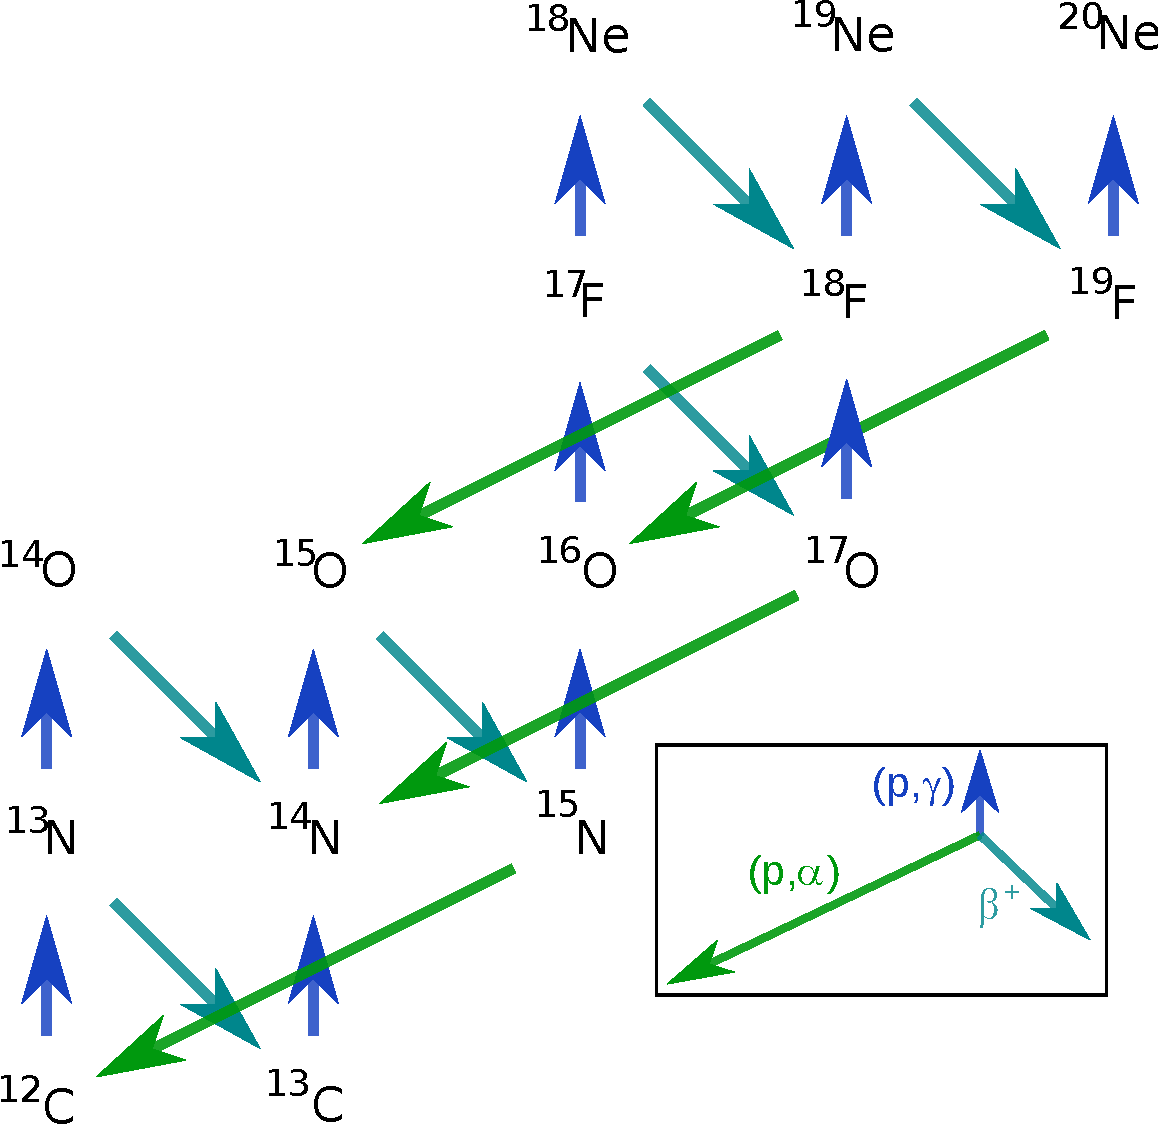
\includegraphics{HotCNO_general.pdf}
}
\caption{The hot CNO cycle.}
\label{fig:hotCNO}
\end{figure}
%
%
\begin{figure}
\centering
\resizebox{0.7\columnwidth}{!}{
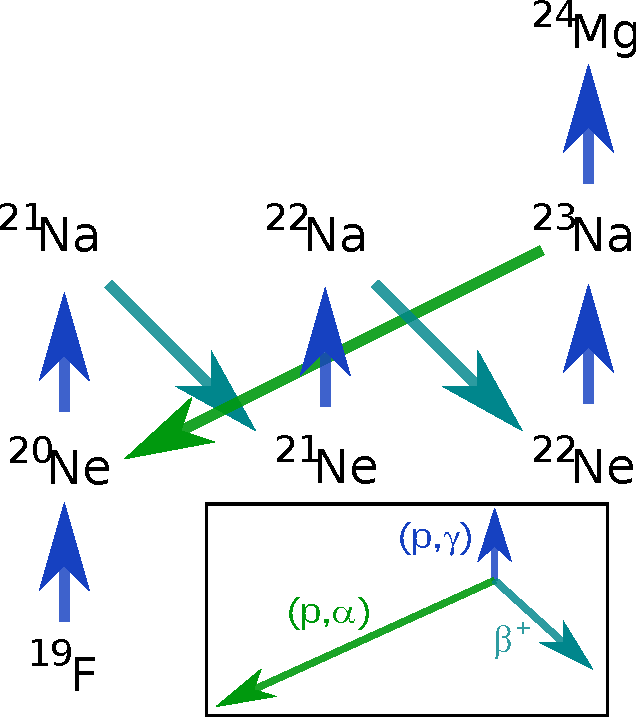
\includegraphics{NeNa-cycle_legend.pdf}
}
\caption{The Ne-Na cycle.}
\label{fig:NeNa}
\end{figure}
%

The proton- and alpha-capture reactions of importance are of critical interest to nuclear experimentalists. Due to the distance from stability and the involvement of few or no isolated narrow resonances, the reaction cross sections cannot be calculated via nuclear models with sufficient accuracy. They must be measured directly or determined partially via indirect experimental methods. This principle founds the basis for many of the experimental nuclear astrophysics programs involved in measuring radiative capture reactions in inverse kinematics.   

\subsubsection{Resonant and direct capture}
\label{resonant}

Radiative capture reactions may proceed through a few different types of mechanisms. These are generally split into {\em direct} and {\em resonant} capture. Direct capture usually occurs as an initial target-plus-projectile state transitioning directly into a bound state via the emission of a $\gamma$ ray, and is a process related to bremsstrahlung in the Coulomb field of the nucleus before subsequent capture (see fig. \ref{fig:radcap}). In some cases, direct capture may occur into an unbound state which subsequently decays to a bound state, see for example, Rolfs and Azuma \cite{rolfs74}. The cross section for direct capture is proportional to the overlap integral (where the radial separation is the variable of integration) of the final bound state with the initial scattering state via the electromagnetic operator. Because in cases where binding energies are low radiative capture reactions at the temperatures of novae and quiescent burning access excitation energies where few or no levels contribute to the cross section, the stellar reaction rate is usually a sum of the direct capture component of the rate plus the contributions from  {\em individual isolated resonances}. Of course broad and overlapping resonances can contribute in some cases, especially when one goes to the cases of higher mass nuclei involved in radiative capture at the kinds of temperatures seen in type I X-ray bursts and supernovae. Most discussions of experimental results in this paper focus on measurements of resonance capture. 

\begin{figure}
\resizebox{0.98\columnwidth}{!}{
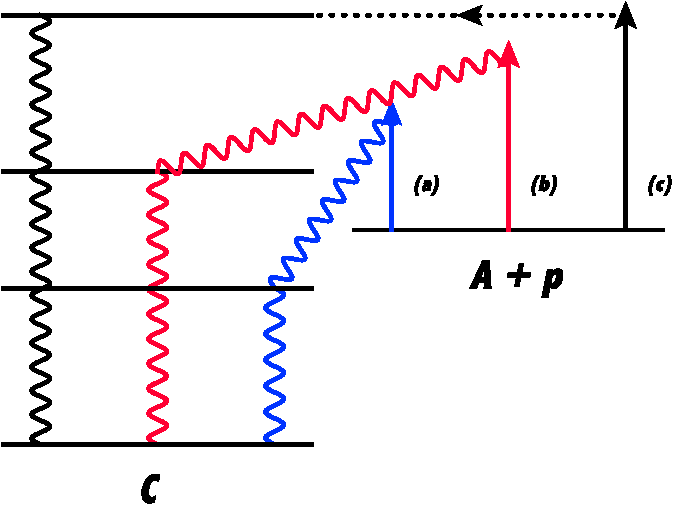
\includegraphics{radcap}
}
%\vspace{5cm}       % Give the correct figure height in cm
\caption{Energy level schematic showing various modes of radiative capture of a proton $p$ by a nucleus $A$ to form a product nucleus $C$. (a) represents direct capture into a bound state, (b) represents direct capture into an unbound (resonant) state, and (c) represents resonant capture into an unbound state.}
\label{fig:radcap}       % Give a unique label
\end{figure}


\subsection{Specifics of inverse kinematics}
\label{specifics}

In inverse kinematics, since the recoiling product nucleus is generally detected, it is important to consider the reaction kinematics in order to understand the final momentum spread and maximum laboratory angle of the recoil. Typical relative energies in the astrophysical regime, for processes occurring in novae and supernovae, can range up to the several hundred keV to MeV range. With typical inverse kinematics accelerated beam energies ranging up to around 2A MeV, the resulting beam velocities are usually below  $\approx0.05c$, and thus relativistic corrections are unnecessary. In the following discussion we will begin with relativistic expressions for kinematic variables for clarity, then reduce to or show alternative non-relativistic expressions where useful. We will also adopt the convention of {\em natural units} where the speed of light is equal to unity.

\subsubsection{Recoil and gamma ray energy and momentum}

In the inverse kinematics radiative capture reaction, the beam particle with laboratory energy $T'_{1}$ and mass $m_{1}$ is incident on the target particle of mass $m_{2}$, forming an excited compound nucleus with mass $m^{*}_{3}=m_{3}+E_{x}$. From energy conservation, it follows that the kinetic energy in the laboratory frame of the excited recoil is $T'^{*}_{3}=T'_{1}-E$ (the asterisk denoting the excited state), i.e. the laboratory kinetic energy of the beam minus the relative centre-of-mass energy of the beam+target. Thus, since subsequent emission of a gamma ray can only remove energy from the system, the kinetic energy of the recoiling nucleus is {\em always} smaller than the beam energy. If the ratio of beam to target mass is large, the recoil energy can be only a relatively small amount lower than the beam energy, a fact that becomes important for recoil separation techniques to be discussed later. 

The excited recoil nucleus then decays via emission of one or more gamma rays. In this example we will consider only one such decay to the ground state. Before the decay, by conservation of linear momentum, the excited nucleus has momentum  equal to that of the incident beam momentum: $(\vec{P}'_{3})^{*}=((E'_{3})^{*},0,0,(p'_{3})^{*})=\vec{P}'_{1}$, where we use the relativistic 4-momentum formalism, and define the z-axis to be the incident beam particle axis.  

The gamma ray is emitted (see fig. \ref{fig:kinematics}) in the C.M. system at an angle $\theta_{\gamma}$ w.r.t the z-axis (unprimed quantities are in the C.M. system). Since the recoil moves in a direction in the centre-of-mass system opposite to the gamma ray, we can combine the x- and y-coordinates and talk instead of the momentum components along the z-axis $(z)$ and perpendicular to the z-axis $(\perp)$. Thus the gamma ray will have momentum equal to $\vec{P}_{\gamma}=(E_\gamma, \vec{p}_{\gamma \left( \perp \right)}, p_{\gamma \left( z \right)})$,  while the recoil will have momentum  $\vec{P}_{3}=(E_{3},\vec{p}_{3 \left( \perp \right)},p_{3 \left( z \right)})$. To transform into the laboratory system we use the Lorentz transform equations\footnote{Note that the transformations are into the laboratory frame, which is moving in the direction of negative $z$ w.r.t. the beam direction from the point of view of an observer in the C.M. frame, hence the {\em inverse Lorentz transform} form of the equations are used.}:  

\begin{equation}
E'_{i}=\gamma(E_{i}+Vp_{i \left( z \right)})
\end{equation}
\begin{equation}
p'_{i \left( z \right)}=\gamma(p_{i \left( z \right)}+VE_{i})
\end{equation}
\begin{equation}
\vec{p}'_{i \left( \perp \right)}=\vec{p}_{i \left( \perp \right)}
\end{equation}
%
where $V=(p'_{3})^{*}/(E'_{3})^{*}$ is the velocity of the centre-of-mass system and $\gamma=(E'_{3})^{*}/m^{*}_{3}$ is the relativistic factor. 

These can be used to derive an exact expression for recoil kinetic energy:

\begin{equation}
\label{eqn:recoilenergy}
T'_{3}=\gamma(\sqrt{m_{3}^{2}+E_{\gamma}^{2}}-VE_{\gamma}\cos{\theta_{\gamma}})-m_{3}
\end{equation}
%
Evaluating this at $\theta_\gamma = \pi / 2$ and expanding the relativistic factor, $\gamma$, we get the {\em central kinetic energy} of the recoil:

\begin{equation}
T'_{3}=\frac{T'_{1}+Q+m_{2}}{m_{3}+E_{x}}\sqrt{m_{3}^{2}+E_{\gamma}^{2}}-m_{3}
\end{equation}

We can derive a similar expression for the laboratory gamma ray energy:

\begin{equation}
E'_{\gamma}=\gamma E_{\gamma}(1+V\cos{\theta_{\gamma}})
\end{equation}
%
and for the laboratory gamma ray angle:

\begin{equation}
\tan{\theta'_{\gamma}}=\gamma^{-1}\frac{\sin{\theta_{\gamma}}}{\cos{\theta_{\gamma}}+V}
\label{eqn:thetagamma}
\end{equation}
%
The latter two equations effectively show the Doppler effect on the gamma ray, resulting in a change in photon wavelength and direction in the laboratory frame. This effect also has the result of pushing flux in the backwards and forwards C.M. hemispheres forwards when transformed into the laboratory frame, resulting in a slight preference for flux in the forward laboratory frame. This has implications when considering to use gamma-ray hit-pattern information to deduce the reaction spatial origin in extended targets, as we shall see later on.  

\begin{figure}
\resizebox{1.0\columnwidth}{!}{
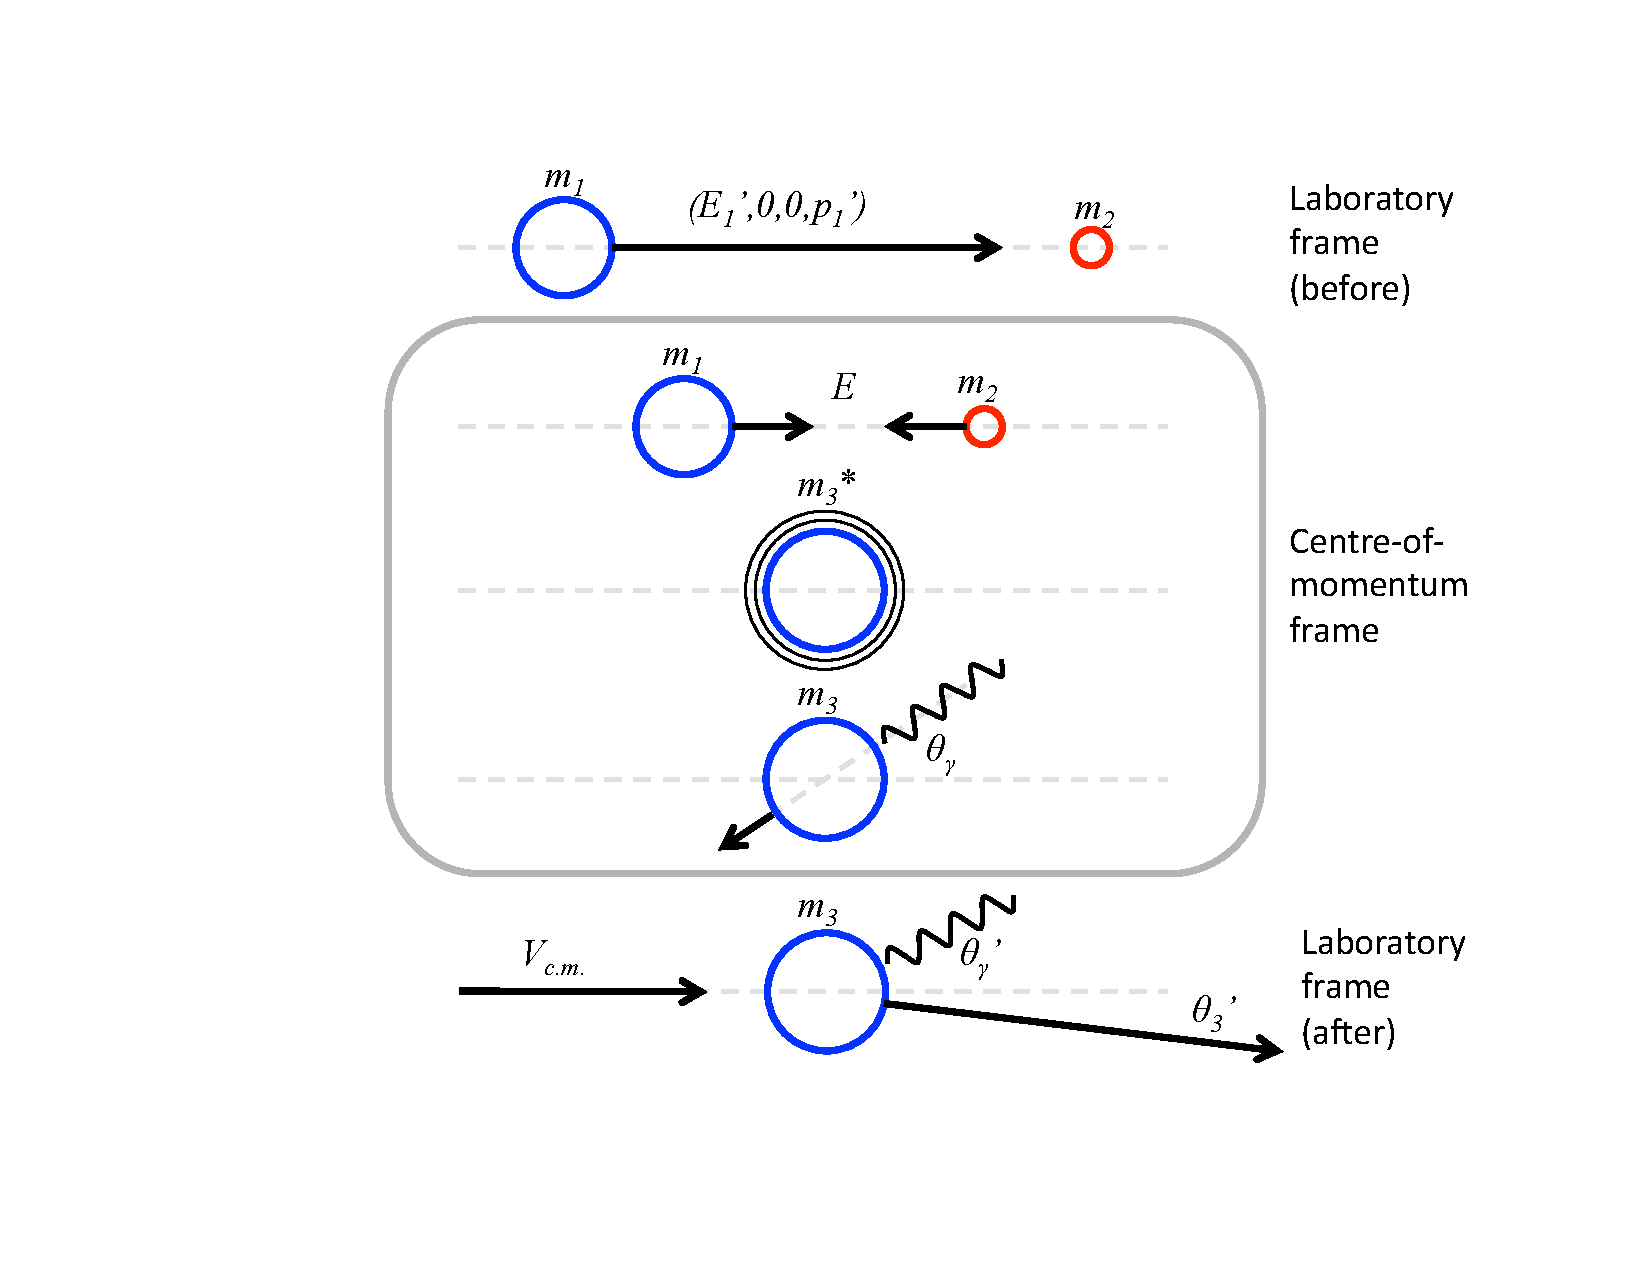
\includegraphics{kinematics}
}
%\vspace{5cm}       % Give the correct figure height in cm
\caption{Simplified schematic of kinematics of radiative capture reaction.}
\label{fig:kinematics}       % Give a unique label
\end{figure}

In addition, we can consider the momentum spread of the recoiling nucleus in order to quantify what range of momenta must be accepted in the recoil separator. Now, in the non-relativistic approximation, the maximum momentum spread of the recoil is given by the approximate relation:

\begin{equation}
\frac{\Delta p'_{3}}{p'_{3}}\simeq\frac{E_{\gamma,max}}{p'_{1}}\simeq\theta'_{3,max}
\end{equation} 

Thus a recoil separator designed to study the recoil products of such a reaction would need to accept momenta with $p'_{3}(1\pm\frac{\Delta p'_{3}}{p'_{3}})$. For typical beam velocities ranging from $(0.1-1.5)A\cdot$MeV at accelerator facilities interested in direct measurements, and for nuclei of interest in the range A=10-40, beam momenta can take on values anywhere between some hundred to over one thousand MeV/c. With reaction Q-values in the range anywhere from under an MeV to 10 MeV, in principle momentum spreads can take on values from fractions of one percent to several percent. Any recoil separator designed to measure such reactions must identify the range of reactions and meet the specifications for momentum acceptance therein.  

\subsubsection{Recoil angular distribution}

Returning to the Lorentz transformation expression, we can derive a similar expression to that of equation \ref{eqn:thetagamma} for the recoil particle:

\begin{equation}
\tan{\theta'_{3}} = \frac{\sin{\theta_{3}}}{\gamma(V/v_{3}+\cos{\theta_{3}})}
\end{equation}
%
Here, $v_{3}$ is the recoil velocity in the centre-of-mass frame given to the product nucleus due to the emission of the $\gamma$ ray, and $\theta_{3}$ is the angle of the recoiling nucleus in the centre-of-mass frame with respect to the incident beam particle direction. The maximum recoil angle that can possibly occur is when the energy of the emitted $\gamma$-ray is maximized ($E_{\gamma}=Q+E$), where $E$ is the relative energy of target and projectile in the centre-of-mass\footnote{ $E=\sqrt{2m_{2}(T'_{1}+m_{1})+m_{1}^{2}+m_{2}^{2}}-m_{1}-m_{2}$, and in the non-relativistic approximation $E=\frac{m_{2}}{m_{1}+m_{2}}T'_{1}$ }, and the emission occurs perpendicular to the incident beam direction ($\theta_{3}=\pi/2$) so that:

\begin{equation}
\tan{\theta'_{3,max}}=\frac{v_{3}}{\gamma V}
\end{equation} 
%
It can be shown that in the non-relativistic limit this can be approximated by:

\begin{equation} \label{eq:6}
\tan{\theta'_{3,max}}\simeq\frac{Q+E}{\sqrt{2\frac{m_{1}}{m_{2}}(m_{1}+m_{2})E}}
\end{equation}
%In the following discussion we assume a projectile of mass $m_{1}$, momentum $p_{1}$ and kinetic energy $T_{1}=p_{1}^{2}/2m_{1}$ is incident on a stationary target particle of mass $m_{2}$.   
%The relative energy in the centre-of-mass system is given by:\footnote{The fully relativistic expressions are: $T_{1}=\sqrt{p_{1}^{2}+m_{1}^{2}}-m_{1}$ and $E_\mathrm{c.m.}=\sqrt{2m_{2}(T_{1}+m_{1})+m_{1}^{2}+m_{2}^{2}}-m_{1}-m_{2}$, with all energies in units of MeV and all masses in units of MeV/$c^{2}$.  }
%
%\begin{equation}
%E_\mathrm{c.m.}=\frac{m_{2}}{m_{1}+m_{2}}T_{1}
%\end{equation} 
It is interesting to note that this relation has a minimum ($\frac{d\theta'_{3,max}}{dE}=0$) when $E=Q$. Figure \ref{fig:coneangles} shows the maximum recoil half-angle in the laboratory frame versus centre-of-mass energy, for a variety of astrophysically interesting radiative capture reactions. As shown by equation \ref{eq:6}, the position of the minimum and therefore the local behaviour of the functions is determined by the reaction $Q$-value. For example the $^{7}$Be($p,\gamma$)$^{8}$B reaction which has a $Q$-value of only $0.138 \unit{MeV}$, generally has the maximum recoil half-angle increasing with increasing centre-of-mass energy above this value. On the other hand the $^{23}$Na($p$,$\gamma$)$^{24}$Mg reaction, with $Q=11.693 \unit{MeV}$, generally has its maximum recoil half-angle decrease with increasing beam energy over the astrophysically relevant energy range. This has implications for the geometric acceptance of recoil separators built to study such reactions. 

Of course the above discussion only tells us what the maximum possible recoil angle is in the event that the entire centre-of-mass energy is converted by emission of a single gamma ray to the recoil ground state, and says nothing of the distribution of the recoil directions. In the event of a multiple-gamma cascade, each decay will proceed in some direction in the centre-of-mass system resulting in a recoil laboratory polar angle less than the maximum possible in a single decay. In rare occasions the momentum vectors of these decays can line up to reach the equivalent of a single gamma ray, but more usually they will be unaligned, with the probability of alignment dropping rapidly with the number of gamma rays in the cascade. The result is that the most probable recoil angle, or the mean recoil angle, will be less than the maximum angle. In addition, the in-target angular straggling and divergence of the incoming beam will in general broaden the resulting distribution.
To illustrate this, Figure \ref{fig:26altheta} shows a kinematic simulation for resulting recoil polar angles for the $^{26}$Al($p,\gamma$)$^{27}$Si reaction on the $E_{c.m.}$=188 keV resonance, originating at the centre of an extended gas target, using realistic values of incident beam energy spread, transverse emittance and straggling. Shown are two different cases, one where the gamma decay from the resonating $^{27}$Si state goes 100$\%$ to its ground state, the other where the decays proceed through a series of cascades, with no gamma decay direct to the ground state. The maximum recoil polar angle allowed by kinematics in such a case is 15.6 mrad, however the incident beam properties mentioned above conspire to increase this maximum slightly. 
One can immediately see from the figure that for a finite angular acceptance recoil separator or detector cutting into the angular distribution, the effect on detection efficiency is much more severe in the case of 100\% ground state decay than in the case of the cascade. It is thus important to know the branching ratios of such decays in advance if the angular acceptance of the recoil separator/detector is close to the maximum recoil angle. If branching ratios are completely unknown, simulations can determine efficiencies, and combined with detected gamma ray information, can lead to a determination of branching ratios.    

\begin{figure}
\resizebox{\columnwidth}{!}{
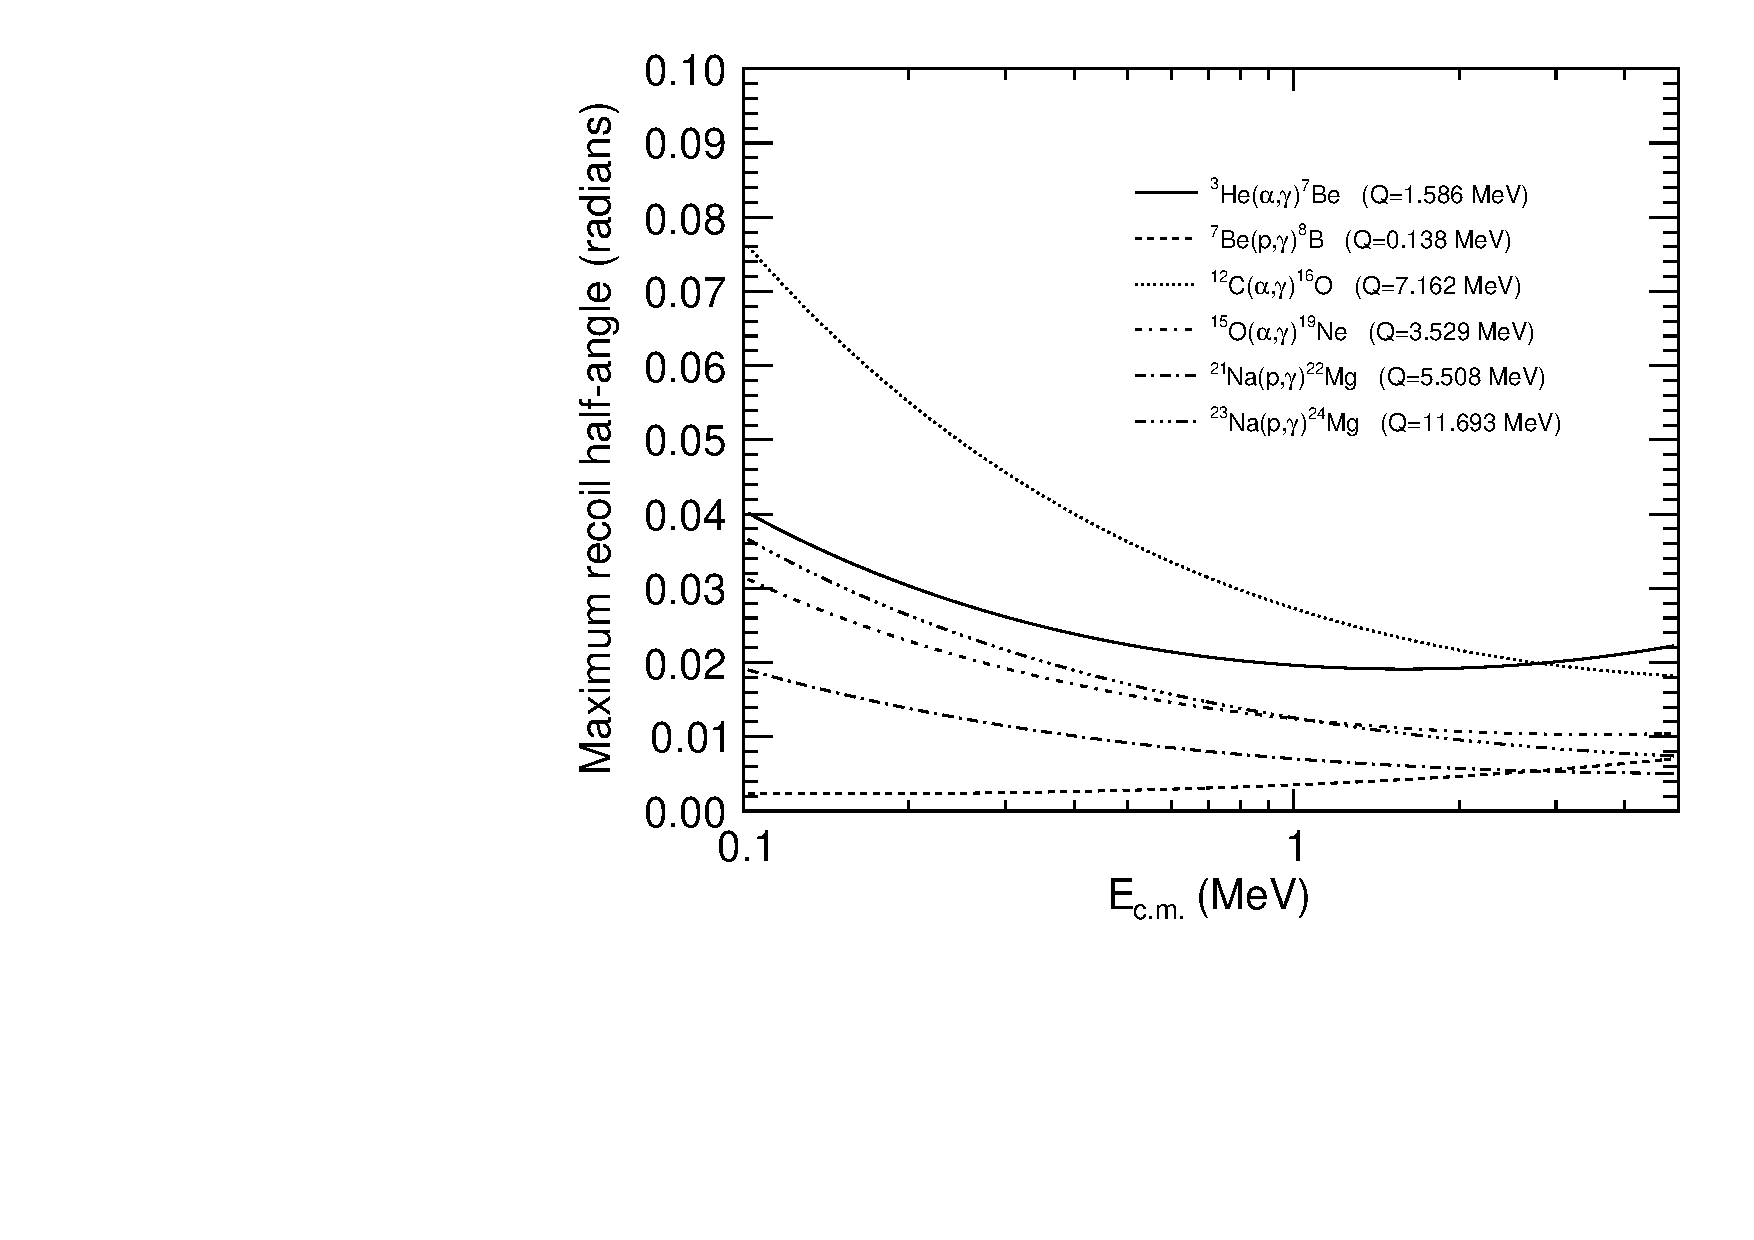
\includegraphics{coneangles}
}
%\vspace{5cm}       % Give the correct figure height in cm
\caption{Maximum recoil half-angle as a function of centre-of-mass energy, for a variety of interesting radiative capture reactions.}
\label{fig:coneangles}       % Give a unique label
\end{figure}

\begin{figure}
\resizebox{\columnwidth}{!}{
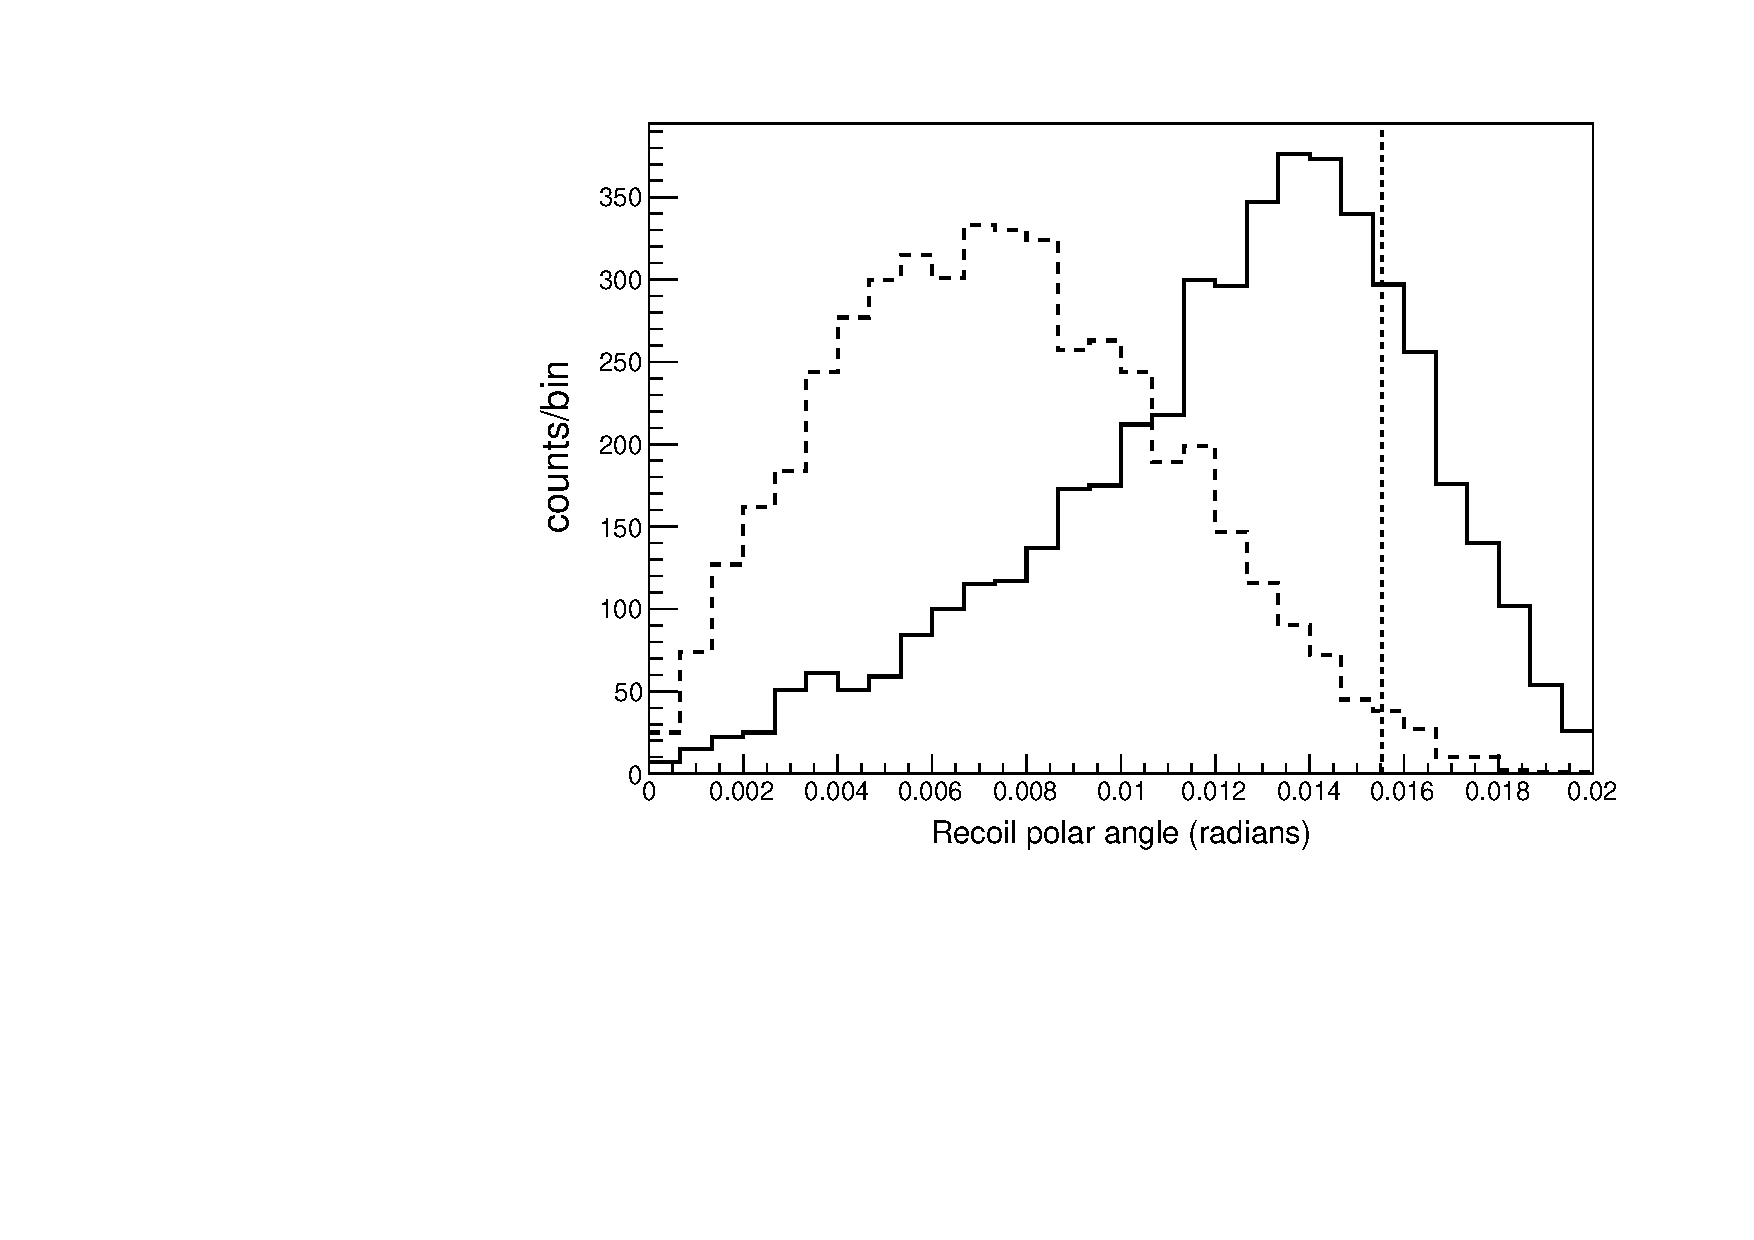
\includegraphics{26altheta}
}
\caption{Hypothetical inverse kinematics distribution of recoil angles emerging from the $^{26}$Al($p,\gamma$)$^{27}$Si reaction at $E_{c.m.}$=188 keV in an extended gas target, using realistic values of beam emittance, energy spread, and straggling (isotropic gamma ray angular distribution in the C.M. system). The solid histogram shows the case where 100\% of decays are to the ground state; the dashed histogram shows the case for a series of cascade gamma rays. The dotted line shows the maximum possible recoil angle in the case of perfectly aligned incident beam particles. }
\label{fig:26altheta}       % Give a unique label
\end{figure}

\subsubsection{$\gamma$-ray angular distribution and effect on recoil angle and energy} 

The angular distribution of the gamma rays in the centre-of-mass system also plays a role in determining the recoil angular (and energy) distribution. Since we are considering the effect on the recoil angular distribution, we are talking here about the cumulative effect of several gamma rays in a cascade. In principle, this depends in a complicated fashion on the spins of the nuclear levels and the multipole mixing ratios of the gamma transitions. For simplicity, we consider the case where the initial transition is to the ground state or to a very low-lying excited state, so that subsequent transitions (if any) have negligible impact on the momentum of the heavy recoil particle. In addition, most of the low energy radiative capture reactions interesting for astrophysics will proceed via low orbital angular momentum transfer into a resonant state. For direct capture the situation can be complicated and is not considered here, but for individual narrow resonances, states of definite $J^{\pi}$ are populated.

For s-wave proton capture, the distribution of initial $\gamma$ decays will be isotropic in the centre-of-mass frame. This is because it is clear that when $\ell=0$ the compound nuclei are formed with no preferred axis, as the unpolarized initial beam and target spins combine randomly. Thus although each {\em individual} $\gamma$ decay (which can in principle be an admixture of multipolarities) will certainly have some non-uniform angular distribution with respect to the preceding newly-formed spin axis of the excited nucleus, the distribution of directions of all decays will be uniform over a sphere in the centre-of-momentum system. \\
For a single gamma transition to the ground state, the magnitude of the momentum imparted to the recoil is always the same, $E_{\gamma}/c$ where $E_{\gamma}$ is the $\gamma$-ray energy.
In the case of initial s-wave capture into a series of cascade transitions, the magnitude of the vector sum of the decays will differ according to the correlations however.
For example, in a 2-$\gamma$ cascade involving spin sequence $0\rightarrow 1 \rightarrow 0$  the angular correlation takes the form $1+\cos{2\theta}$ and larger or smaller magnitudes of the vector sum of momenta are favoured at the expense of intermediate values.  Conversely, for a spin sequence $1\rightarrow 1 \rightarrow 0$ the correlation is $1-(1/3)\cos{2\theta}$ and the vector sums of intermediate value are enhanced. \\
In summary for s-wave capture by a single $\gamma$ ray to the ground state, the angular distribution will be  isotropic in the centre-of-mass frame, however for cascade transitions, although the summed vectors of the $\gamma$-decays might be random in direction, correlations have an effect on the resulting recoil distribution and thus the recoil energy distribution seen in the laboratory. 

In the case of p-wave proton capture, anisotropy is possible when the spin, $J$, of the resonant state is greater than the sum of the intrinsic spins of the projectile and target. The orbital angular momentum $\ell$ has a component only in the $m=0$ state, with the result that the magnetic substates of the resonant level having projection $M=\pm J$ cannot be populated. The system is not spherically symmetric and the gamma rays show some anisotropy.

The special case of spin-zero projectile and target nuclei, i.e. $\alpha$-capture on a spin-zero nucleus, can result in large anisotropies in the initial $\gamma$-ray angular distribution with respect to the beam axis and thus the recoil angular distribution. This is because the channel spin, $s=0$ and thus the compound nucleus is formed purely by coupling to the orbital angular momentum quantum number, $\ell$. When this is non-zero, it causes the system to align with the momentum vector of the beam nucleus, i.e. the beam axis. Subsequent multipole decay angular distributions will therefore be reflected in the recoil angular distribution with respect to the beam axis. Strong dipole and quadrupole distributions can be found for example in the recoil energy spectra from resonances in the \nuc{12}{C}\reac{\alpha}{\gamma}\nuc{16}{O} reaction \cite{mat06}, with the relationship between recoil energy and $\gamma$-ray angle being given by eqn. \ref{eqn:recoilenergy}. 

%\subsection{Experimental requirements theory of separators, and figures of merit}

%\small
%\begin{itemize}
%\item Do we want to do an opening angle figure ( opening angle as a function of mass with different lines for different max Eg = Q+ Ecm emitted)?
%\item Recoil separator capable of accepting the recoil angle of the specific reaction targeted
%\item combination of recoil separator and focal plane detector capable of separating beam and reaction recoils
%\item additional use of g-detector array
%\item what are typical: g-ray energies (multiplicity); momentum distribution; opening angles; target thickness; geometry; stopping; straggling; charge state distributions
%\item Is there a time structure of the beam; other beam properties; what are the minimum beam properties needed?
%\end{itemize}
%\normalsize
